
\chapter*{Benchmarks and simulation framework}
\label{sec:org2740419}

In this chapter we describe the benchmarks that will be mapped to the surface code chip and the framework develop for the study of the mapping metrics.

\section*{Benchmarks}
\label{sec:org5fe30ac}
As stated in the Introduction, the research was conducted to analyze the different metrics to assess the quality of a mapping algorithm.
To this purpose, we selected a set of quantum algorithms available in the literature.

We built a list of quantum algorithms coming from different sources.
The sources we chose are RevLib \cite{Wille_2008}, ScaffCC \cite{JavadiAbhari_2015}, some benchmarks from Zulehner's et al. work \cite{zulehner17:effic_method_mappin_quant_circuit} and QLib \cite{Lin_2014} because of the variety of algorithms and because they are already decomposed in the Clifford+T set.
Note the language used to describe the algorithm varies from source to source.
Although, they all are a QASM-based language, there are small syntax differences.
As we will explain the next section, we will use our own programming languages -- OpenQL -- and compiler.
Therefore we had to translate algorithms from their QASM versions to the OpenQL notation.
We developed a parser in order to do that.

We also built a benchmark profile that includes: the number of qubits of the algorithm, the number of gates, the functionality of the algorithm and different graphs, showing the percentage of the operations types or the degree of parallelism of the algorithm.
Most of the benchmarks are classical algorithms adapted to quantum circuits.
They are deterministic and the result it is always the same if there are no errors.
This means that their results are always binary.
Or what is the same, qubits in either ground or excited state, but never superposition.


The benchmarks were also classified depending on their functionality.
This is an important step because algorithms that do similar calculations are used to have common gates distribution.
From all the benchmarks we have, we can distinct six different classes.

\begin{itemize}
\item Quantum Gates: Circuits that are a decomposition of a Quantum Gate
\item Search Algorithms
\item Worst Cases: Circuits that were really difficult to generate for RevLib
\begin{itemize}
\item HWB: is the simplest function with exponential Ordered Binary Decision Diagrams (OBDD) size.
\end{itemize}
\item Encoding Functions: Classical codification functions
\item Arithmetic Functions: Functions that perform an arithmetic operation
\item Miscellaneous: Mix of different kind of algorithms
\end{itemize}

We came up with a list of 84 different algorithms -- 697 benchmarks taking into account the different versions of the same functionality -- that can be found in the \href{https://github.com/QE-Lab/qbench}{qbench Github repo}, as well as the previous information much more detailed.
These algorithms cannot only be used for the mapping problem but also for the other activities in our group.

\subsection*{Benchmark selection}
\label{sec:org97a7e3c}

In order to have a small, but representative, set of benchmarks to map, we selected just some of them.
This requirement comes by the fact that simulations are long and computationally exhaustive.
In order to do that, we studied the different benchmark profiles looking for most illustrative cases.
But we also set some restrictions.
First of all, as soon as we are going to map the algorithms to the SC chips with a maximum number of 17 qubits, we need to look for the benchmarks with an amount of qubits below that.
We also want to see how different gate quantities affect the mapping.
Therefore, we need benchmarks with a number of gates as spread as possible.
And, at the same time, several benchmarks presenting the same number of gates.
We also tend to mix all the classes equally.
And we try to have the less number of the same algorithm versions as possible.
We only take the same algorithm versions for cases in which the number of qubits and the number of gates show an interesting combination.
For example, two similar algorithms which number of qubits or number of gates are very distinct as the first three selected benchmarks in Tab. \ref{tab:map_selected_benchs}.

Once we had our requirements we could start the analysis and the selection afterwards.
In Tab. \ref{tab:map_selected_benchs} we show the final benchmark selection.
\begin{table}[htbp]
\caption{\label{tab:orgc867dfc}
Restriction summary of the benchmark selection}
\centering
\begin{tabular}{|l|}
\hline
\\
Restrictions:\\
\\
- \# qubits < 17\\
- \# gates as spread as possible and in the case of repeated benchmark the minimum number of gates\\
- The less number of the same algorithm versions/classes as possible\\
- The benchmarks that are repeated and have an interesting combination of No. qubits/No. gates are  preferred\\
\\
\hline
\end{tabular}
\end{table}
43 benchmarks (with qubits numbers from 3 to 17 qubits) selected after applying the previous Restrictions to the analysis of the benchmarks described in the next section (see Table \ref{tab:map_selected_benchs}).
After simulating the algorithms, few of them returned errors (segmentation fault) and some others .

\section*{Simulation framework}
\label{sec:org311b249}
In this section we introduce the framework we developed in order to analyze the quantum metrics.
It is based on two steps: \textbf{compilation} and \textbf{simulation}.
With this purpose we connect two tools, OpenQL and quantumsim, and we build a whole framework over them.

\subsection*{Compiler (OpenQL)}
\label{sec:orgff7c703}
OpenQL is a framework for high-level quantum programming developed by our group.
It is able to describe both, quantum circuits and quantum devices.
The framework can be found as a library in either C++ or Python and, therefore, the circuits are described over one of these programming languages.
The quantum chips and their constrains are described in a JSON file that is imported in the circuit description.
OpenQL is able to compile quantum circuits for specific devices and export a code understandable by a quantum simulator.
One of it's compiler processes is the \textbf{mapper} algorithm developed by our group.
Therefore we will use OpenQL to describe the circuit and compile it for the SC-17 chip.
In Fig. \ref{code:openql_gray_code} we show an example of OpenQL code using Python that describes the Gray encoder quantum circuit (Fig. \ref{fig:circuit_example}).
More insights can be found in the \href{https://github.com/QE-Lab/OpenQL}{github repository}.

\begin{figure}
\centering
\begin{minipage}{\textwidth}

\begin{minted}[frame=lines,fontsize=\scriptsize,linenos,breaklines,breakanywhere]{python}

from openql import openql as ql

def circuit(config_file, scheduler='ASAP', uniform_sched= 'no', mapper='base', initial_placement='no', output_dir_name='test_output', optimize='no', measurement=True, log_level='LOG_WARNING'):
    curdir = os.path.dirname(__file__)
    output_dir = os.path.join(curdir, output_dir_name)
    ql.set_option('output_dir', output_dir)
    ql.set_option('optimize', optimize)
    ql.set_option('scheduler', scheduler)
    ql.set_option('scheduler_uniform', uniform_sched)
    ql.set_option('mapper', mapper)
    ql.set_option('initialplace', initial_placement)
    ql.set_option('log_level', log_level)

    config_fn = os.path.join(curdir, config_file)

    platform  = ql.Platform('starmon', config_fn)
    sweep_points = [1,2]
    num_circuits = 1
    num_qubits = 6
    p = ql.Program('graycode6', platform, num_qubits)
    p.set_sweep_points(sweep_points, num_circuits)
    k = ql.Kernel('graycode6', platform, num_qubits)
    k.gate('cnot',[1,0])
    k.gate('cnot',[2,1])
    k.gate('cnot',[3,2])
    k.gate('cnot',[4,3])
    k.gate('cnot',[5,4])

    if measurement:
	for q in range(num_qubits):
	    k.gate('measure', [q])

    p.add_kernel(k)
    p.compile()

\end{minted}

\caption{OpenQL description in python code describing the Gray code algorithm.}
\label{code:openql_gray_code}
\end{minipage}
\end{figure}

\subsection*{quantumsim}
\label{sec:orge732141}

Quantumsim \cite{O_Brien_2017} is a simulator for superconducting systems and designed to study the SC-17 chip.
Its error model has been induced from the chip's behaviour after several experiments.
Therefore, quantumsim's error model is much more complete for the superconducting case than other general simulators.
Although, at the same time, the detail in its error model makes each simulation computationally harder.
As a matter of fact, quantumsim is able to boost its calculations with a Graphics Processing Unit (GPU).
Quantumsim can be found as \textbf{python library} in its \href{https://github.com/quantumsim/quantumsim}{github repository} with instructions to install it and an overview of how to use it.

\subsection*{Simulation Framework}
\label{sec:orgff13d9b}
\begin{figure}[htbp]
\centering
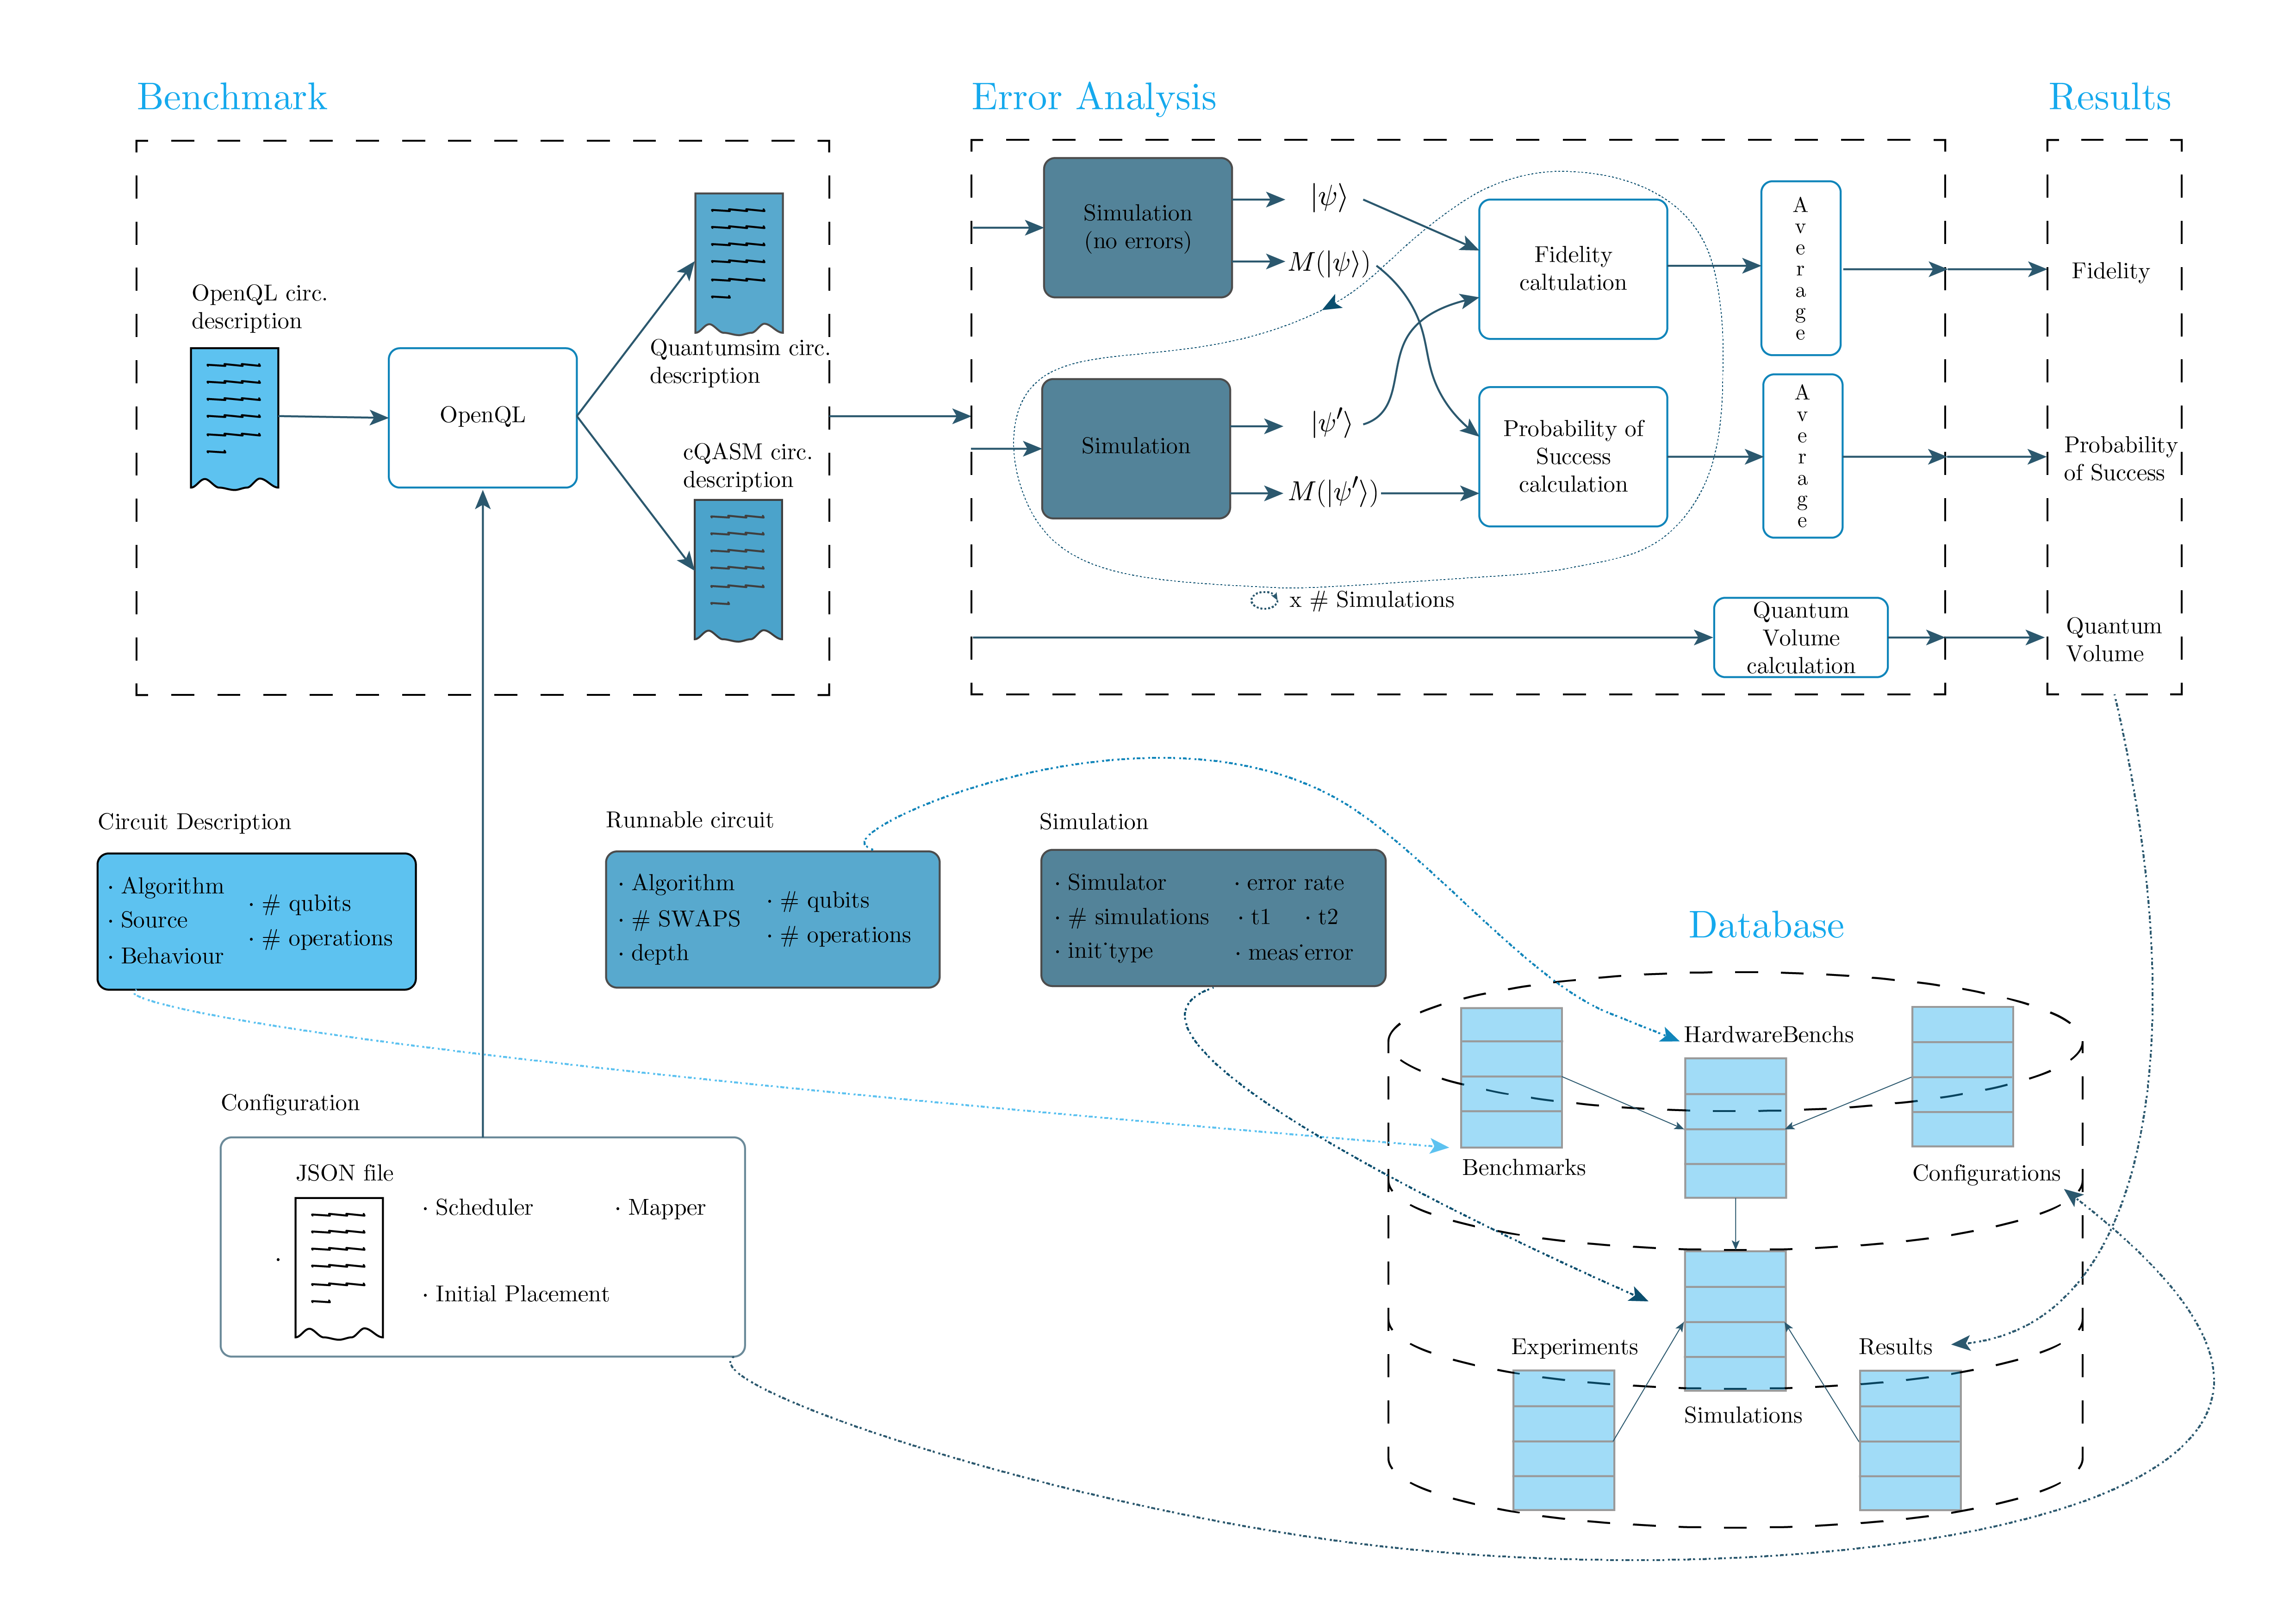
\includegraphics[width=\textwidth]{figures/error_framework_diagram.png}
\caption{\label{fig:org3a0f35c}
Error Framework}
\end{figure}

\begin{itemize}
\item Benchmark Object
\label{sec:orge2b37d9}

\begin{figure}[htbp]
\centering
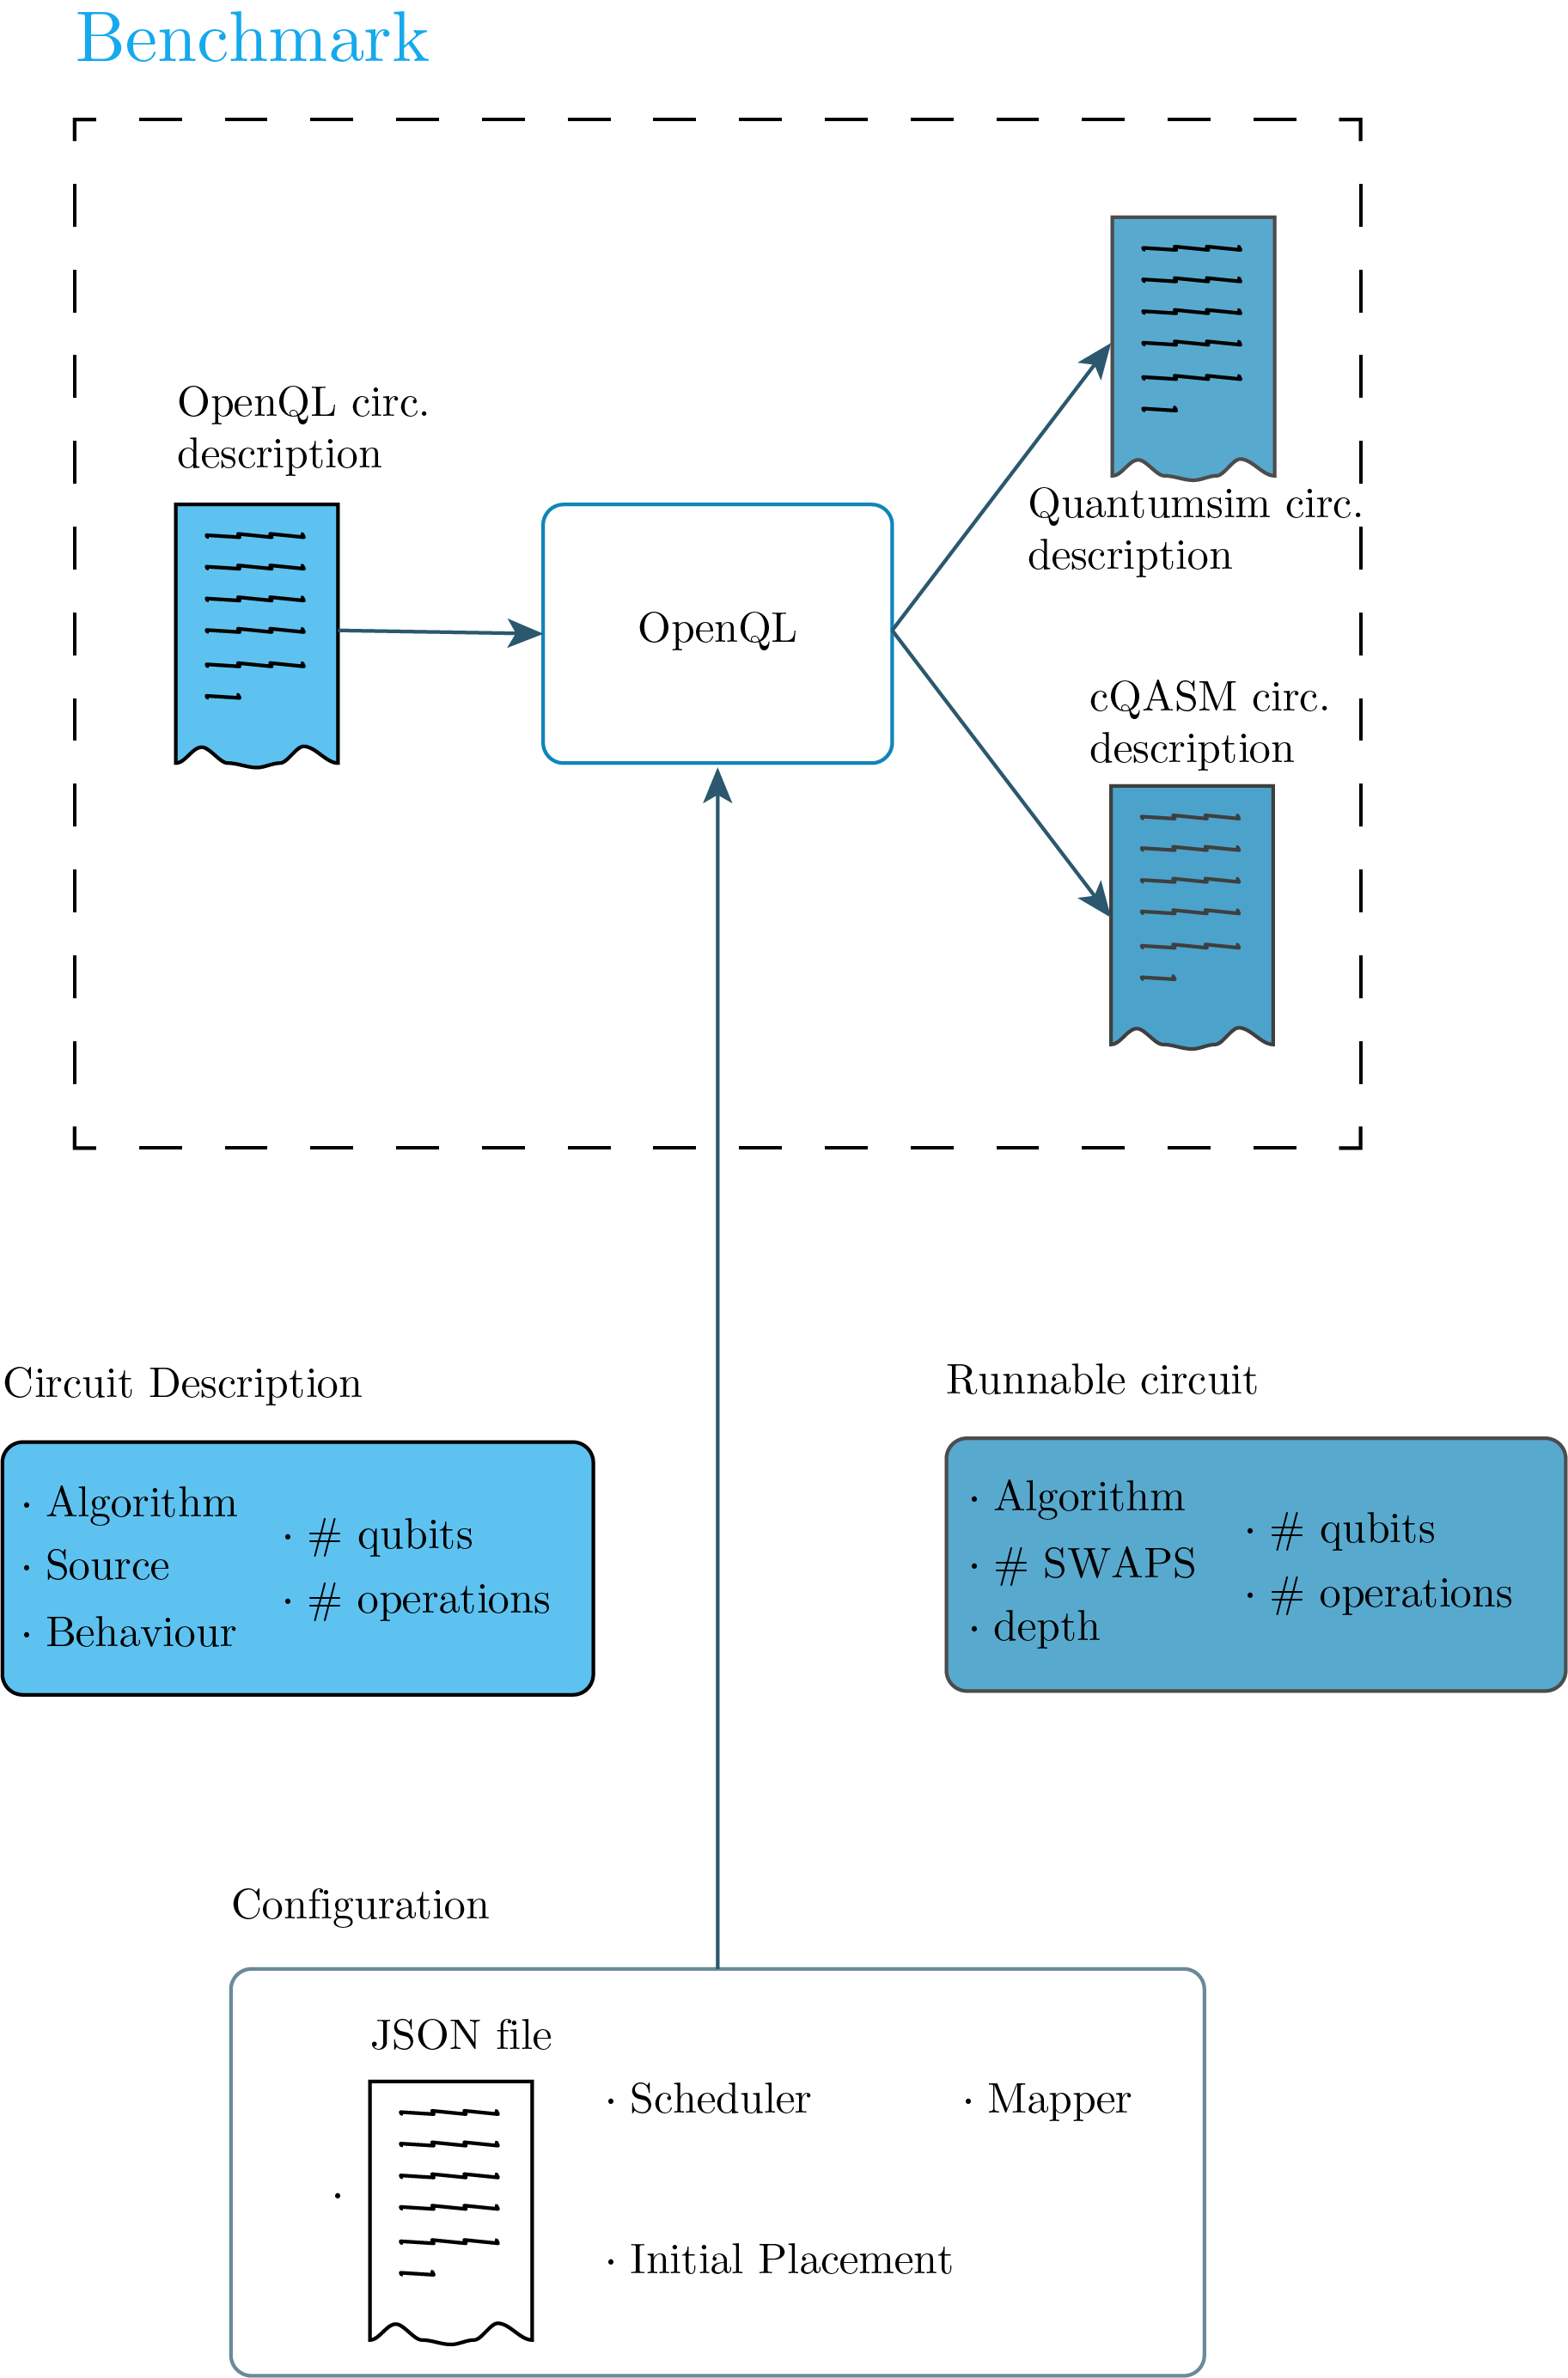
\includegraphics[width=.5\textwidth]{figures/benchmark_object.png}
\caption{\label{fig:orgf8b9852}
Benchmark Object \ldots{}}
\end{figure}

\item Mapping Analysis Object
\label{sec:orgccdac2e}

\begin{figure}[htbp]
\centering
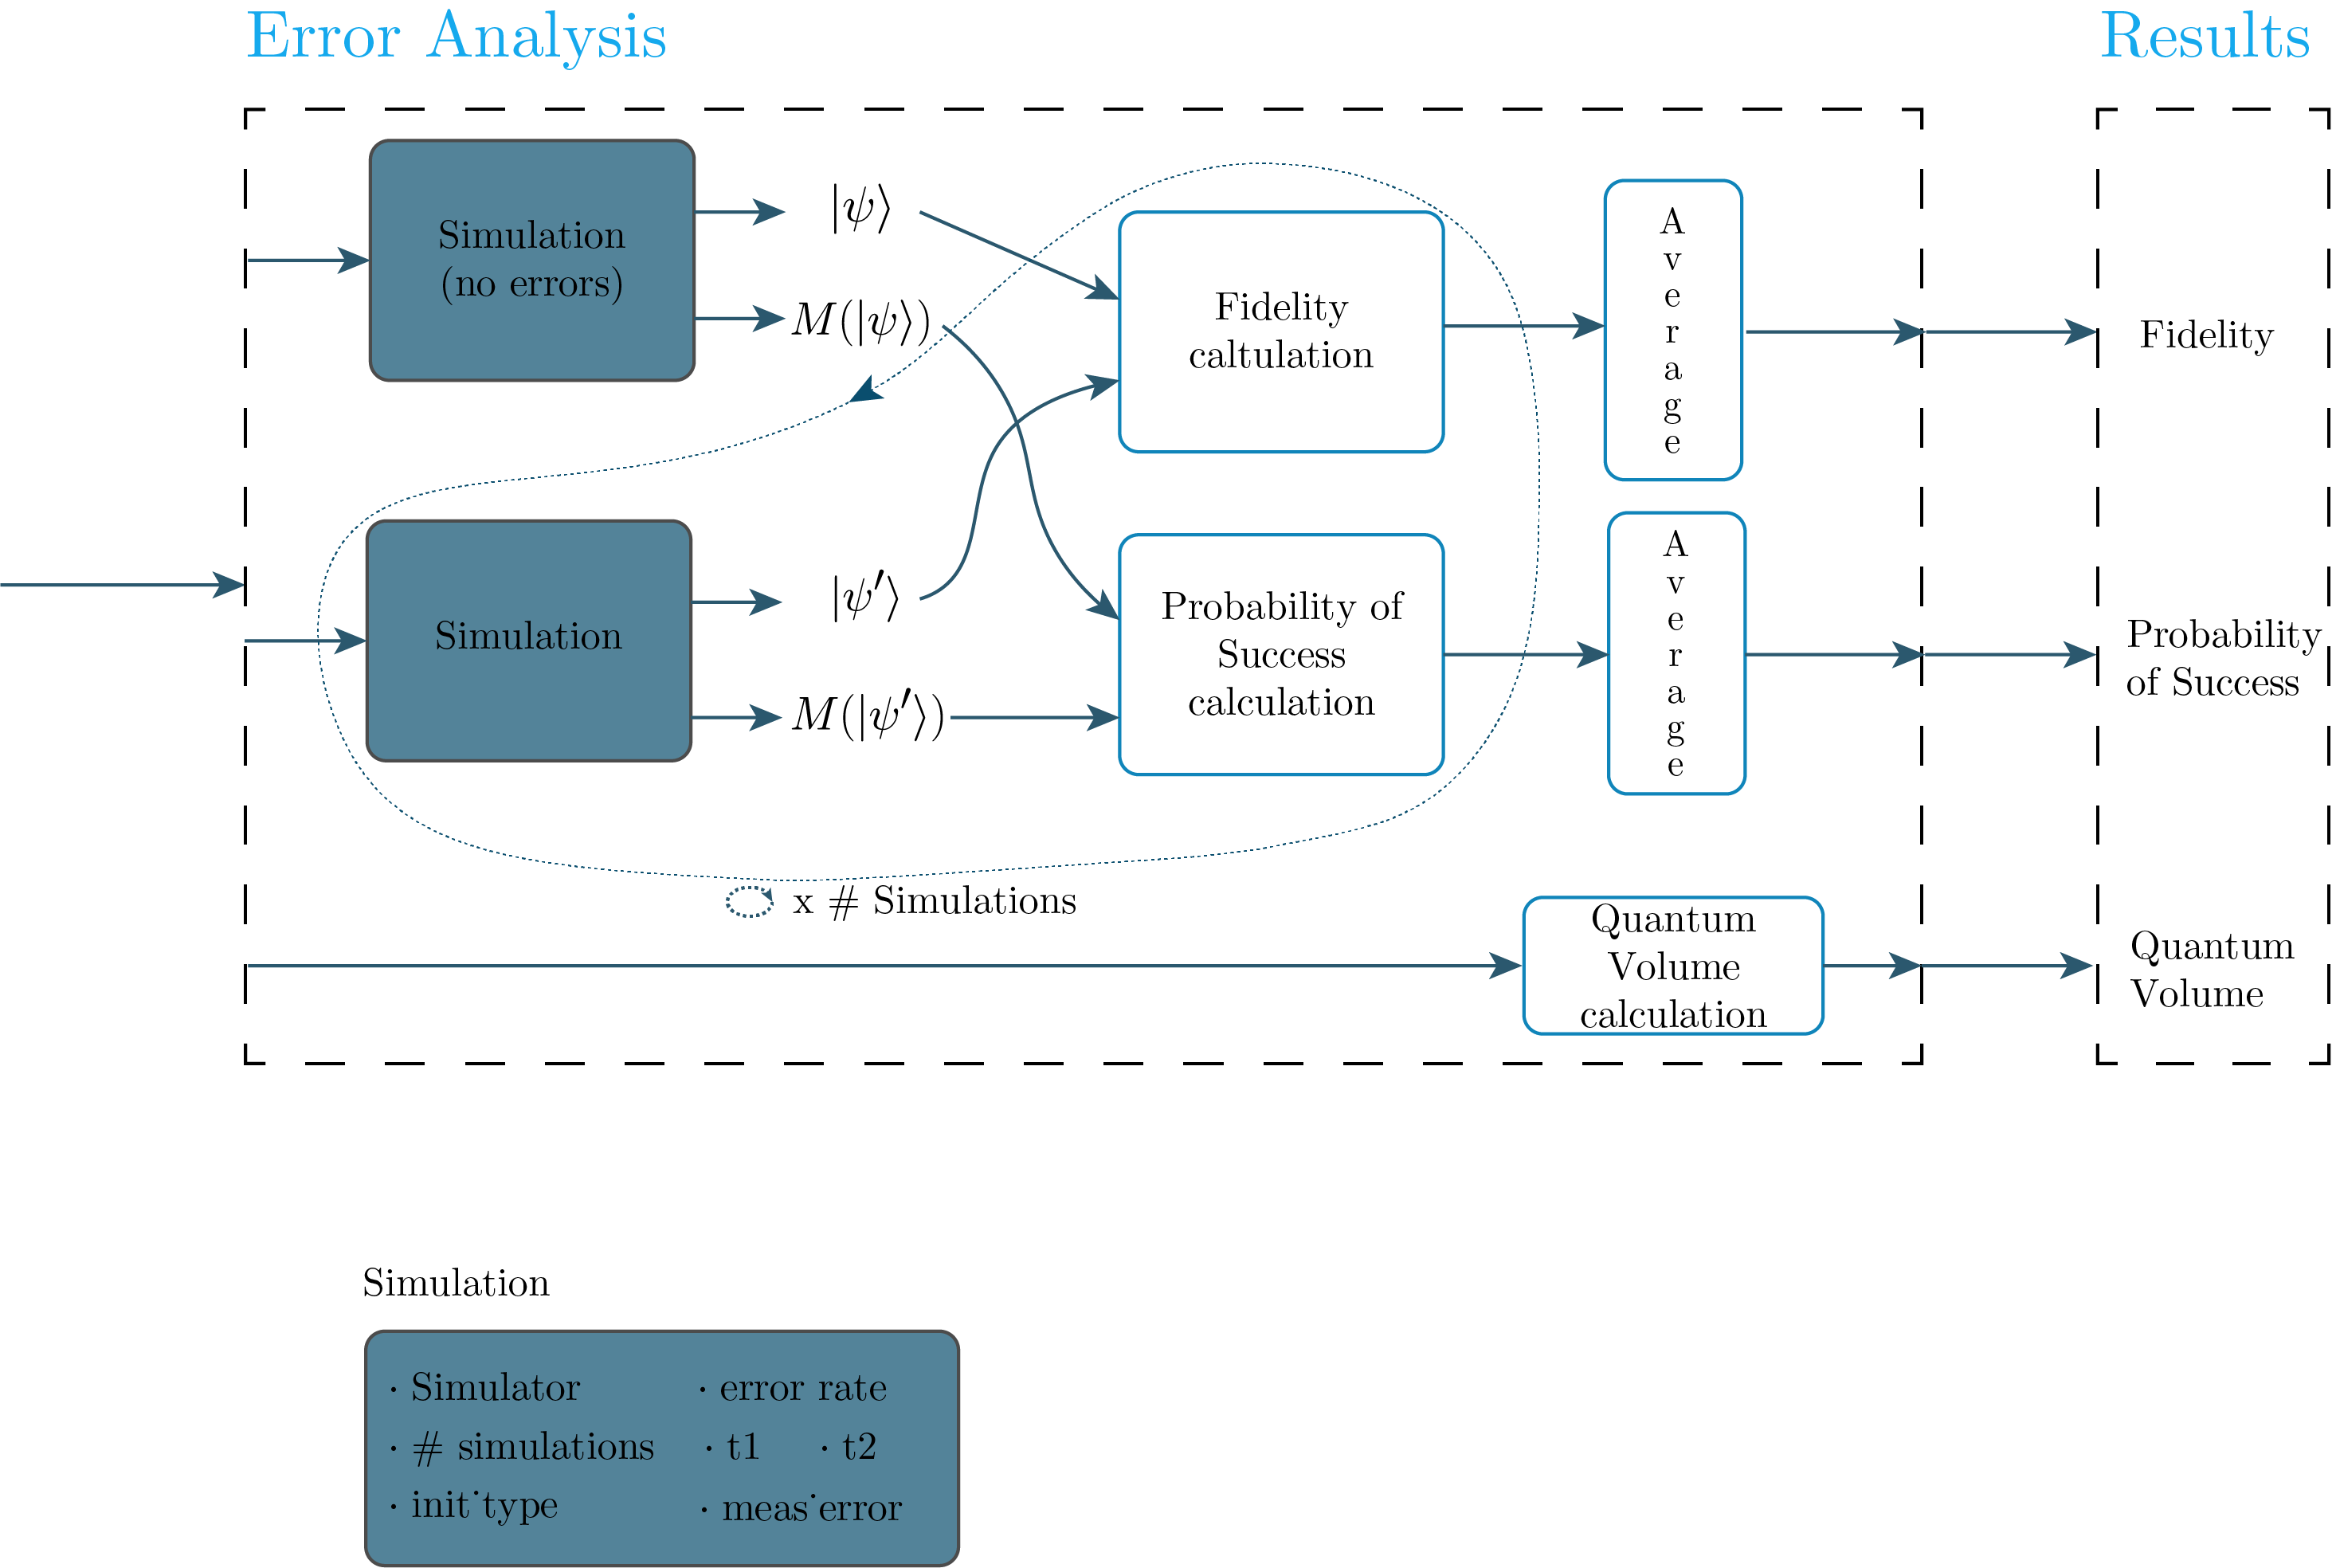
\includegraphics[width=.75\textwidth]{figures/error_analysis.png}
\caption{\label{fig:orge946d9c}
Mapping Analysis Object \ldots{}}
\end{figure}

\item Database
\label{sec:orga307fae}

\begin{figure}[htbp]
\centering
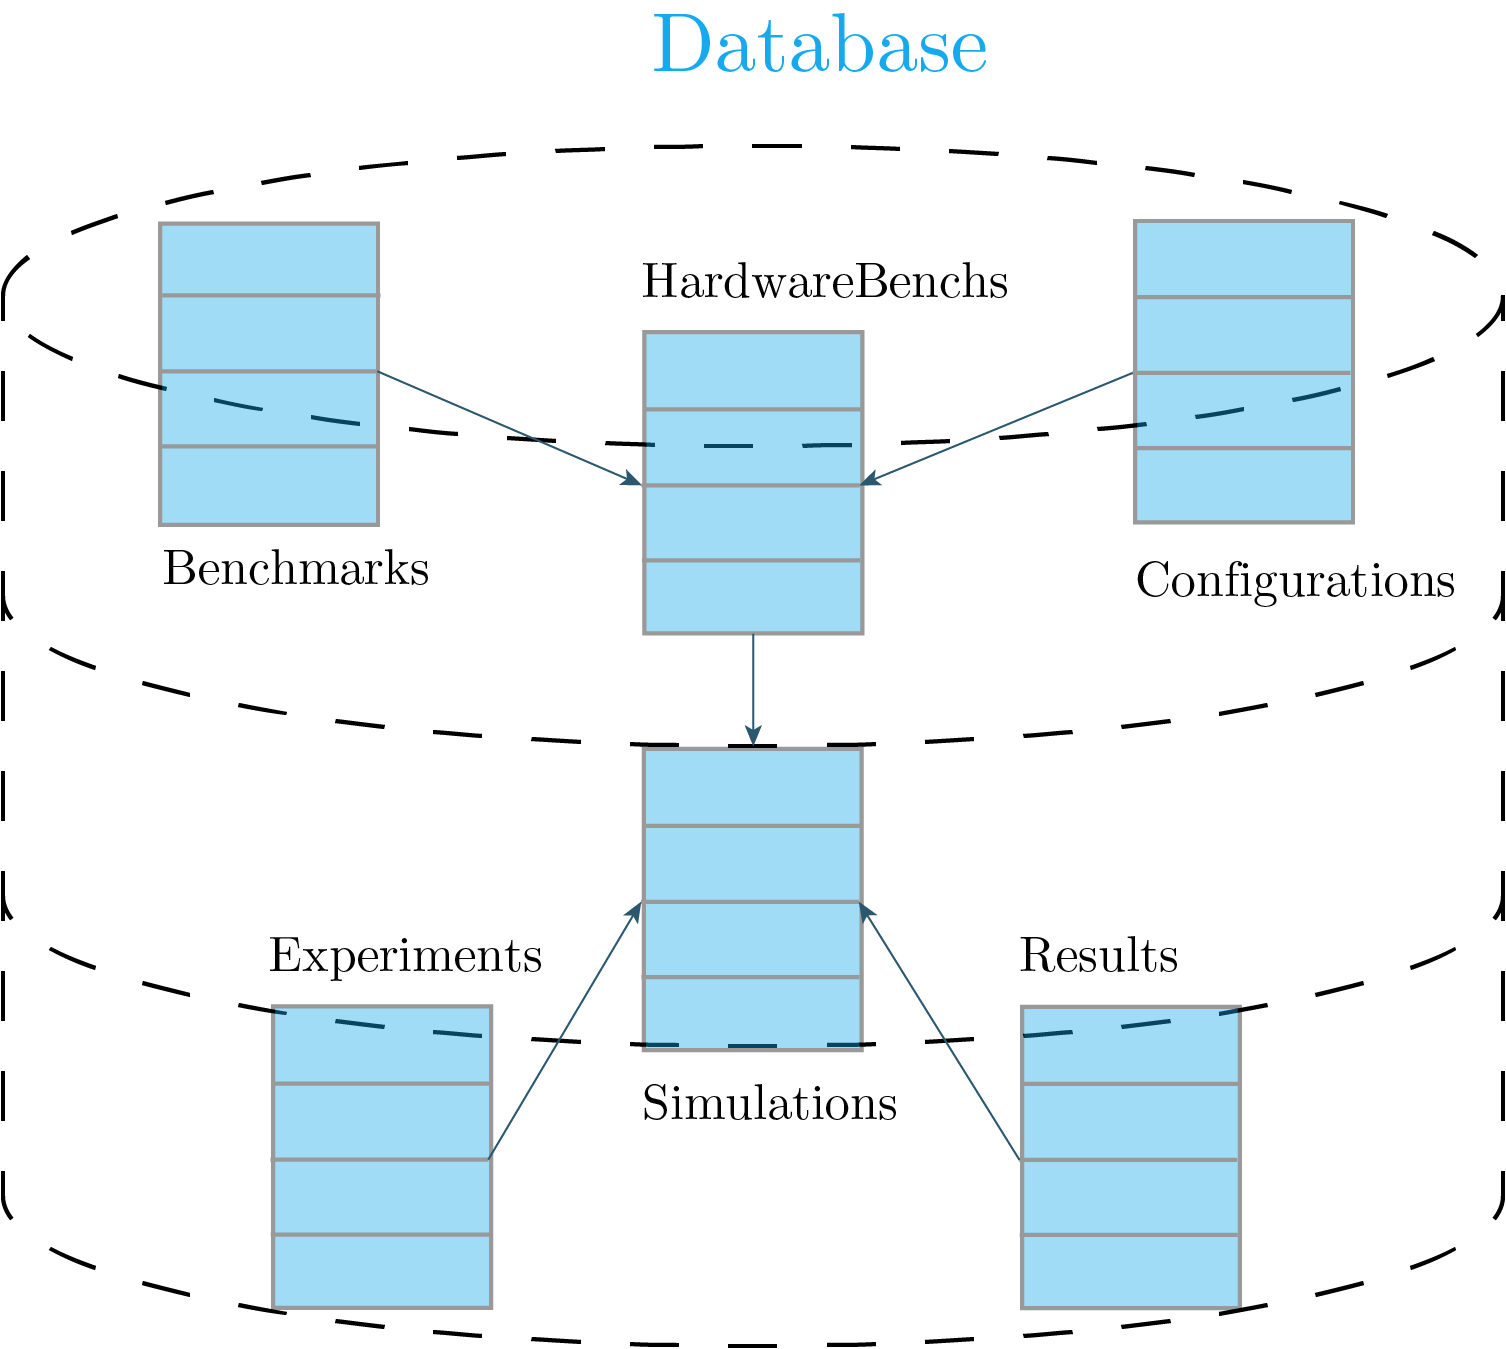
\includegraphics[width=.5\textwidth]{figures/database_scheme_detail.png}
\caption{\label{fig:org8013fae}
Database tables}
\end{figure}

\begin{figure}[htbp]
\centering
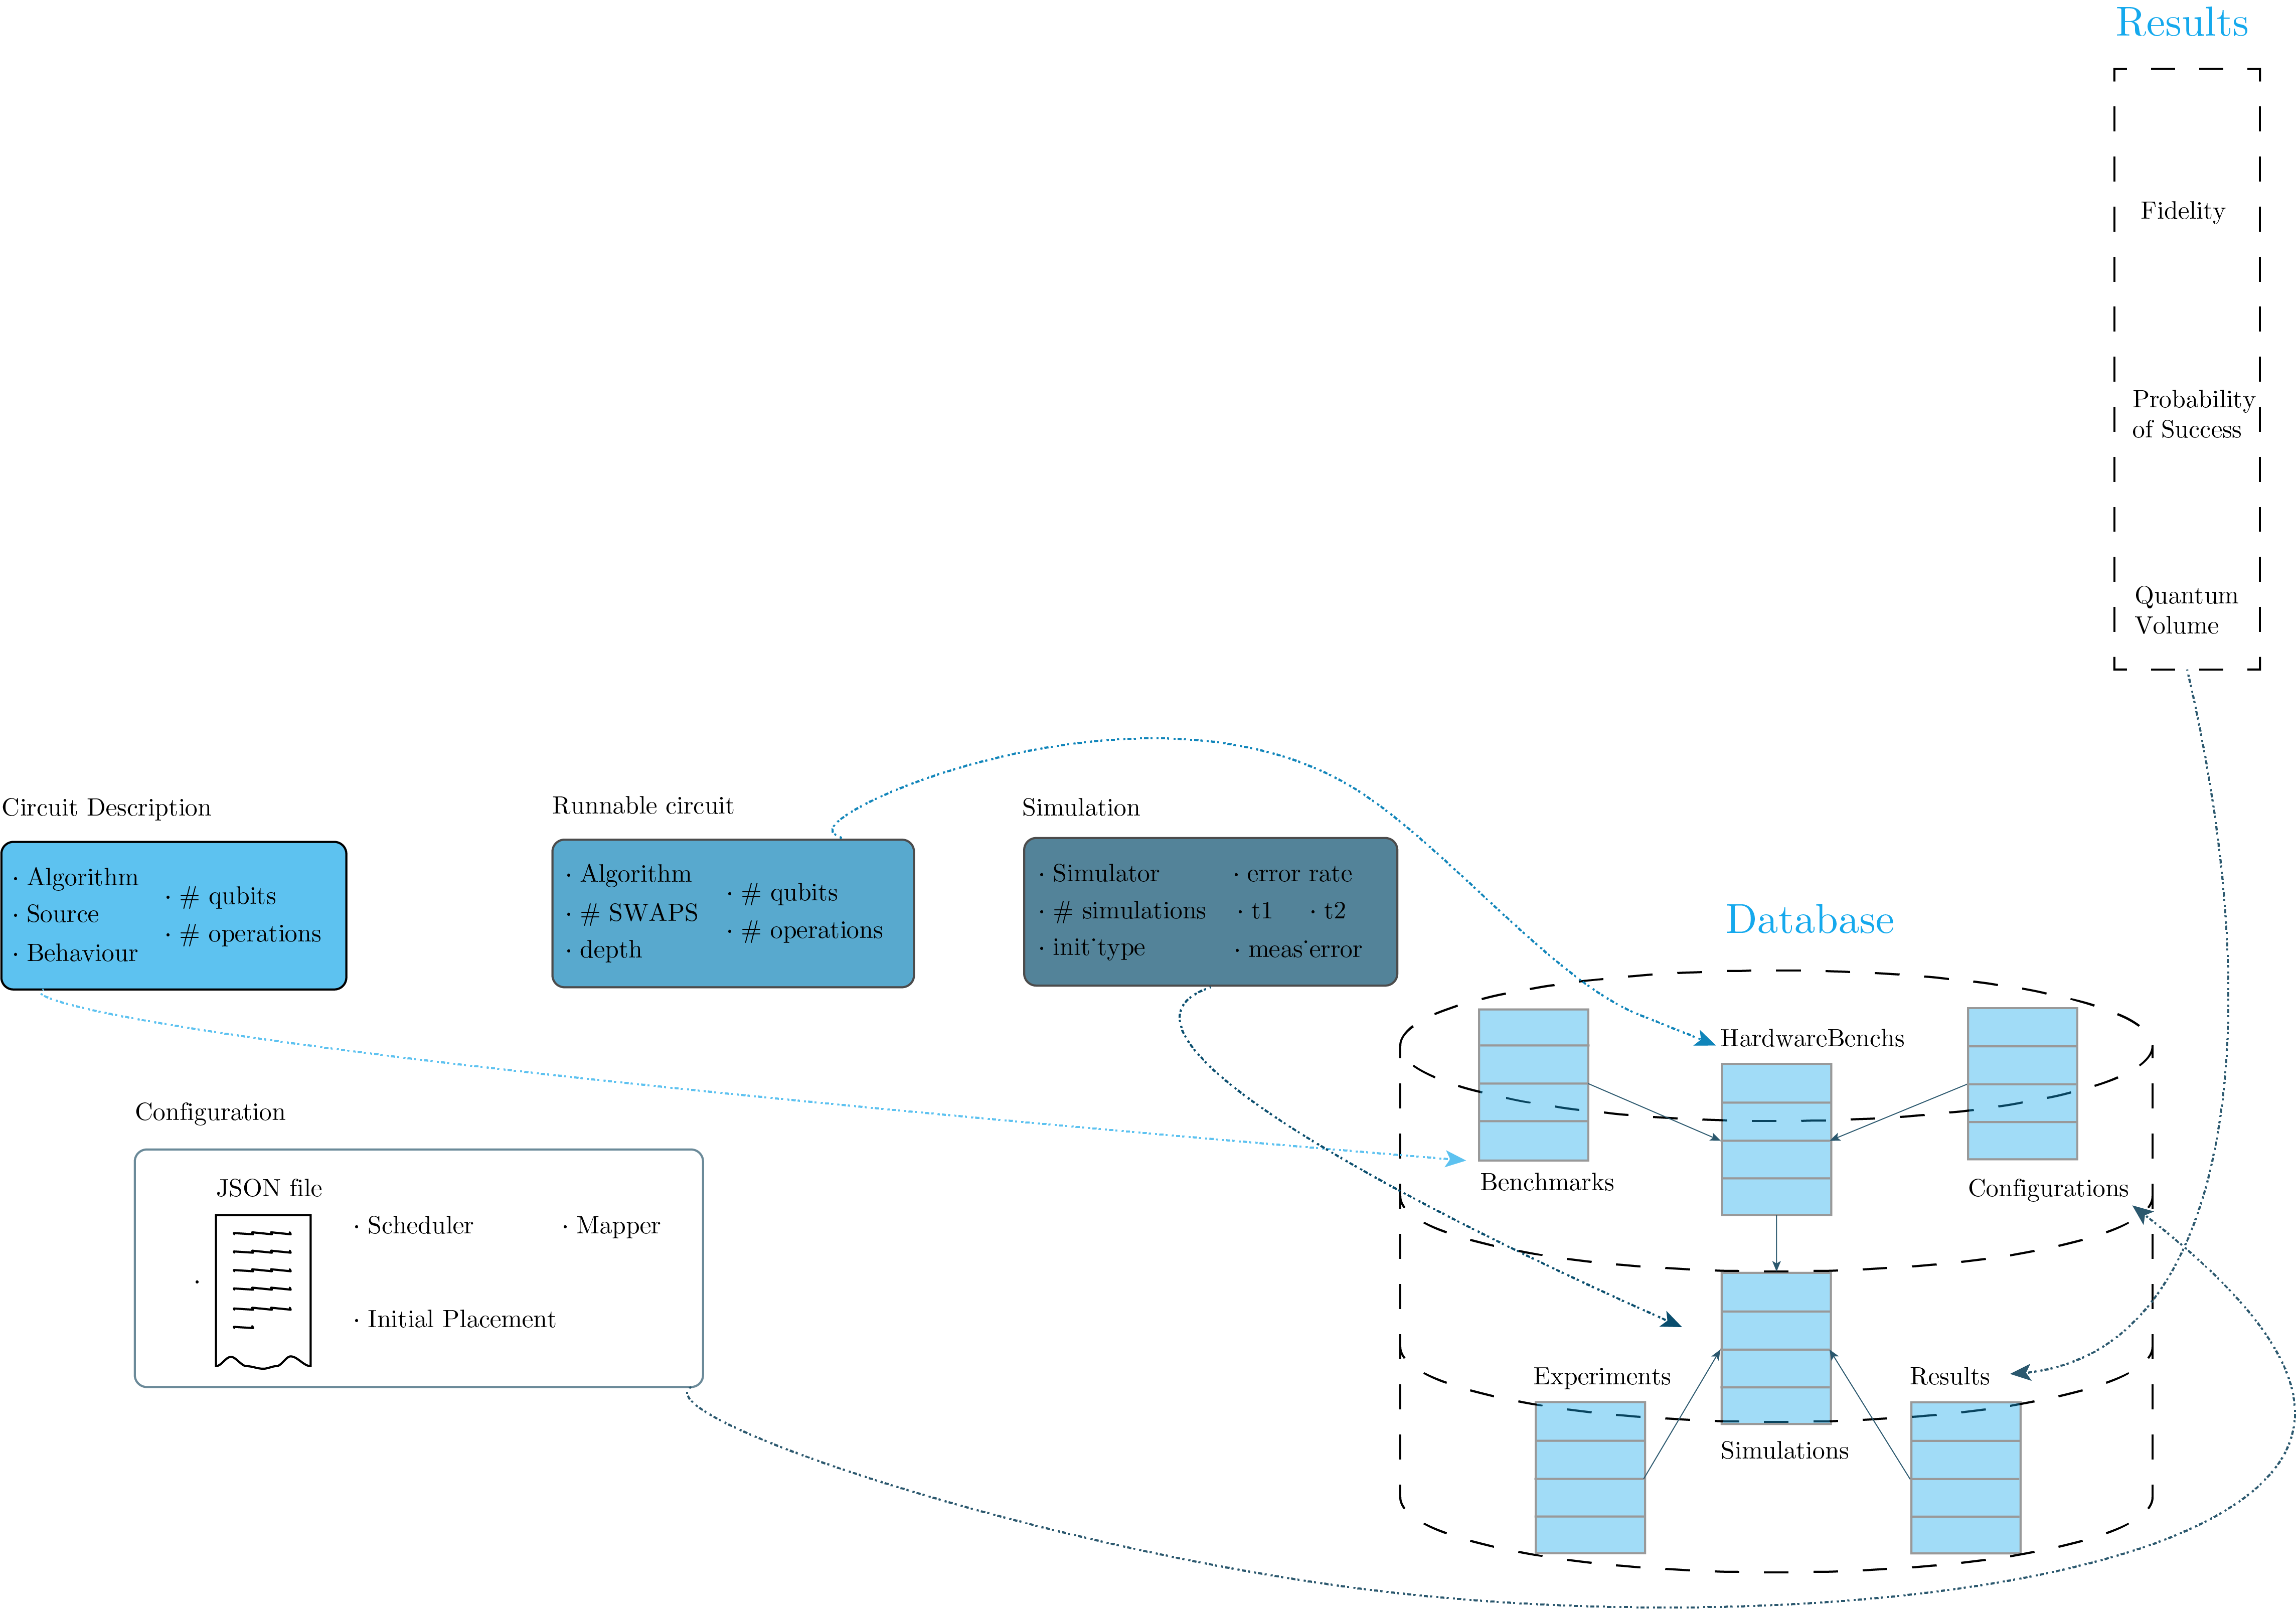
\includegraphics[width=\textwidth]{figures/database_scheme_general.png}
\caption{\label{fig:org18b3601}
Database tables information}
\end{figure}
\end{itemize}
